\documentclass[11pt, a4paper, english]{../Template/NTNUoving}
\usepackage[utf8]{inputenc}
\usepackage[T1]{fontenc}
\usepackage{float}
\usepackage{enumitem}
\usepackage{csquotes}
\usepackage{algorithm}
\usepackage{algorithmic}
\usepackage{listings}
\usepackage{listings}
\usepackage{color}
\usepackage{biblatex}
\usepackage{hyperref}
\ovingnr{3}    % Nummer på innlevering
\semester{Spring 2021}
\fag{Methods in Artificial Intelligence \\ TDT4171}
\institutt{Department for Computer Science}

\begin{document}


% 1
\begin{oppgave}

    %a
    \begin{punkt}
        The decision network can be drawn with decision node $B$ influencing
        $P$ and $M$, $P$ goes into utility node $U_1$, $B$ goes into utility node $U_2$,
        both of these are then again combined into the overall utility node $U$.

        \begin{figure}[H]
            \centering
            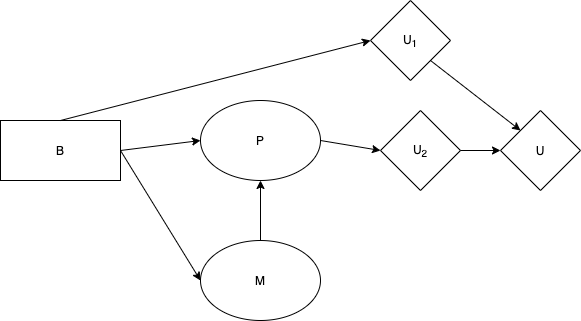
\includegraphics[width=0.8\textwidth]{Task3_1.png}
            \label{fig:1}
            \caption{Decision network for Task 1a.}
        \end{figure}
    \end{punkt}

    %b
    \begin{punkt}

        First we calculate the probabilities of passing ($P$) for both of the decisions:
        $B=true$:
        \begin{align*}
            P(P) &= P(P|B,M)P(M|B) + P(P|B,\neg M)P(\neg M|B) \\
            &= 0.9\cdot0.9 + 0.4\cdot0.1 \\
            &= \frac{17}{20} \\
            \implies P(\neg P) &= 1-P(P) = \frac{3}{20}
        \end{align*}
        $B=false$:
        \begin{align*}
            P(P) &= P(P|\neg B,M)P(M|\neg B) + P(P|\neg B,\neg M)P(\neg M| \neg B) \\
            &= 0.7\cdot0.65 + 0.2\cdot0.35 \\
            &= \frac{21}{40} \\
            \implies P(\neg P) &= 1-P(P) = \frac{19}{40}
        \end{align*}
        Now we have all the probabilities needed to calculate the expected values.

        The expected utility for $B=true$:
        \begin{align*}
            U &= U_1(B=true) + P(P) U_2(P=true) + P(\neg P) U_2(P=false) \\
            &= -150 + \frac{17}{20} 2100 + \frac{3}{20} 0 \\
            &= 1635
        \end{align*}

        The expected utility for $B=false$:
        \begin{align*}
            U &= U_1(B=false) + P(P) U_2(P=true) + P(\neg P) U_2(P=false) \\
            &= 0 + \frac{21}{40} 2100 + \frac{19}{40} 0 \\
            &= 1102.5
        \end{align*}

        Since the expected utility for choosing $B=true$ is higher than $B=false$,
        Geir should buy the book.
    \end{punkt}
\end{oppgave}
\clearpage
% 2
\begin{oppgave}

    \section{Overall model and decision nodes}
    I want to make a decision network for first deciding if I should buy a plane ticket today, and then at the beginning of
    the Easter-holiday decide if I should travel home. It is allowed for me to buy a ticket and not go home. It is also allowed for me
    to go home in the Easter-holiday even if I didn't buy a ticket today, since I can still buy a ticket, although at a lot higher cost (probably).

    In order to decide on these two non-trivial decisions I have modelled how the decisions are influenced observations such as prices on ticket, different corona restrictions, my physical and mental wellbeing,
    how much school work I get done, how they will affect the grades and more.. The overall model is shown in Figure \ref{fig:2}.

    \begin{figure}[H]
        \centering
        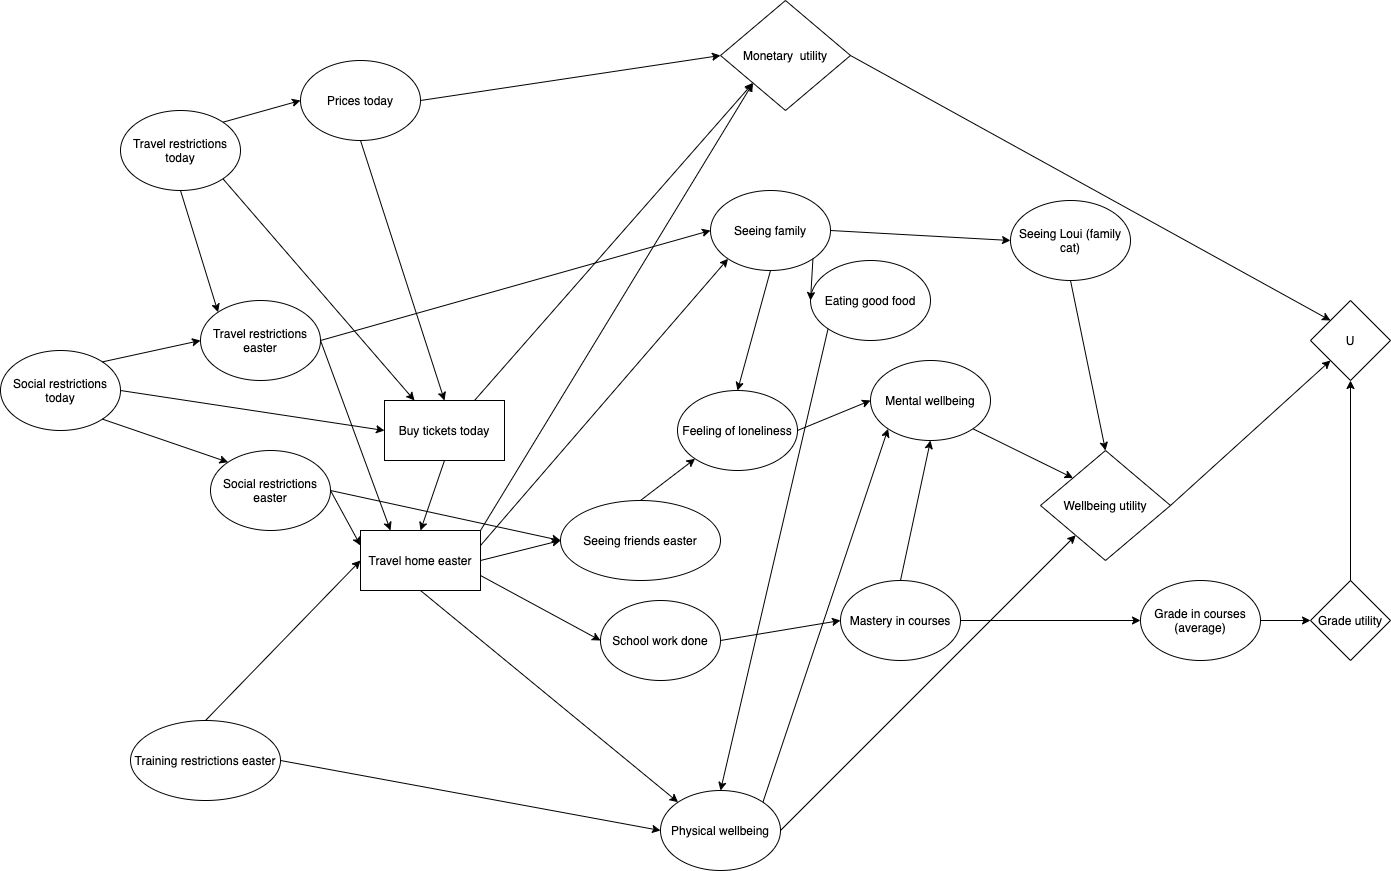
\includegraphics[width=\textwidth]{Task3_2.png}
        \label{fig:2}
        \caption{Decision network for Task 2.}
    \end{figure}

    Now I will go through the thought process behind setting up this complete model and with probability distributions.

    \subsection{How I chose probabilities}
    Choosing how I should assign probabilities was one of the most challenging in this task.
    I decided to use the "fuzzy-logic" approach, by trying to use abstract terms from our language and convert it to a specific
    probability. Whenever I use any of these abstract terms in the text, it is matched with the probability shown
    in Table \ref{tab:prob}

    \begin{table}[H]
        \centering
        \begin{tabular}{|c|c|}
            \hline
            High & $0.8$   \\ [1.0ex]
            Medium & $0.5$   \\ [1.0ex]
            Low & $0.2$   \\ [1.0ex]
            Very Low & $0.05$   \\ [1.0ex]
            Very High & $0.95$   \\ [1.0ex]
            Very Little & $0.1$   \\ [1.0ex]
            Very Much & $0.9$   \\ [1.0ex]
            Not a lot & $0.2$   \\ [1.0ex]
            A lot smaller & $0.05$   \\ [1.0ex]
            Small & $0.3$   \\ [1.0ex]
            Large & $0.7$   \\ [1.0ex]
            Decent & $0.6$   \\ [1.0ex]
            \hline
    \end{tabular}
        \caption{Probabilities for some different abstract terms. }
        \label{tab:prob}
    \end{table}

    This is by no means perfect or an exhaustive list unfortunately, but since this is my own quantitative view of the conversion of these terms into
    probabilities, it is not open to as many misunderstandings as if I where to ask others what probabilities these words should be.

    These probabilities should also be tuned depending on the results I would have gotten with my decision network,
    but I did not do any such analysis as it were not a requirement for the task.


    \subsection{Observational nodes}

    Observations before first decision ($BuyTicketsToday$):
    \begin{itemize}
        \item $TravelRestrictionsToday$
        \item $SocialRestrictionsToday$
        \item $PricesToday$
    \end{itemize}

    Each of these have two discrete states (for simplicity to not make the model overcomplicated):
    \begin{enumerate}
        \item $High$
        \item $Low$
    \end{enumerate}

    $TravelRestrictionsToday$ are here more for the whole country, like when the government told students to not travel to their university for example.
    $SocialRestrictionsToday$ are more local and about how open the city is.

    These were chosen as these are the most influential on my decision to travel, and they influence other nodes in the network.

    The observations before the second decision ($TravelHomeEaster$):
    \begin{itemize}
        \item $TravelRestrictionsEaster$
        \item $SocialRestrictionsEaster$
    \end{itemize}

    These are not observed until after the first decision and for calculational properties we must assign a CPT to each. They are also influenced
    by the previous observations as this makes a lot of sense, as higher restrictions now will make it less probable to have restrictions later.
    The CPTs can be found in Table \ref{tab:obs1} and \ref{tab:obs2}.

    \begin{table}[H]
        \centering
        \begin{tabular}{|c|c|c|}
            \hline
            $TravelRestrictionsToday$ & $SocialRestrictionsToday$ & $P(TravelRestrictionsEaster=High)$ \\ [0.5ex]
            \hline
            $High$ & $High$ & 0.4  \\ [1.0ex]
            $High$ & $Low$ & 0.5  \\ [1.0ex]
            $Low$ & $High$ & 0.6  \\ [1.0ex]
            $Low$ & $Low$ & 0.7  \\ [1.0ex]
            \hline
    \end{tabular}
        \caption{Probability distribution for $TravelRestrictionsEaster$.}
        \label{tab:obs1}
\end{table}

\begin{table}[H]
    \centering
        \begin{tabular}{|c|c|}
            \hline
            $SocialRestrictionsToday$ & $P(SocialRestrictionsEaster=High)$ \\ [0.5ex]
            \hline
            $High$ & 0.3  \\ [1.0ex]
            $Low$ & 0.6 \\
            \hline
    \end{tabular}
        \caption{Probability distribution for $SocialRestrictionsEaster$.}
        \label{tab:obs2}
    \end{table}


    \subsection{Uncertain non-observational nodes}
    The decision of travelling home is the decision which influences most of the non-observational uncertain nodes.
    As I want to measure the utility as a function of overall wellbeing and the monetary value (e.g. money spent), the uncertain nodes
    is a way to see how the decision and evidence influences my overall wellbeing.

    I have tried doing this by setting up the uncertain nodes:
    \begin{itemize}
        \item $SeeingFriendsEaster$: The probability for seeing my friends in easter, for me it doesn't really matter if I want to meet 1
        or more so this is for me a boolean uncertainty. This node is influenced whether I travel home, as I am more likely to meet friends at home and by the
        social restrictions in easter as more social restrictions makes it less likely that I can meet my friends.
        \item $SeeingFamily$: The probability of seeing my family. This is influenced by both the travel restrictions and whether I travel home.
        As my hometown is far away from Trondheim, the probability of me seeing my family should be very low if I don't travel home. Travel restrictions will also influence this node since there
        is always a chance that my family could go see me, even if I don't travel home.
        \item $SeeingLoui$: Probability of me seeing our family cat Loui. Make an assumption that it is independent of travel restrictions and travelling home given if I see my family since our cat is pretty much always taken care of by my family.
        Even if I see my family there is still a chance that I don't see our cat. If I don't see my family the chance of seeing Loui should be close to 0, but it is still possible.
        \item $SchoolWorkDone$: The probability of me having done my school work as a boolean state. This is influenced by both if I meet my friends and if I meet my family, because I obviously
        will not have as much time on my hand if I meet them.
        \item $MasteryInCourses$: The probabilities of three different states of mastering the courses: $High$, $Medium$, $Low$. This is only influenced by the amount of school work done, so I made the conditional independence assumption
        that given school work done, it doesn't depend on if I have met friends or family.
        \item $GradeInCourses$: This is the probability distribution over three possible states: A-B, C-D, E-F. This is meant as an average over all my courses, as having one node for each course would make the network exponentially larger for little reason. I assume that this is independent of all other factors given my mental wellbeing and mastery in courses,
        as this makes the most sense to me, it is only the influence of mentall wellbeing/mastery which really affects the grades, not whether I see my family/friends etc.
        \item $FeelingLonely$: This is the probability that I will feel lonely given as a boolean state, as this is usually how I perceive it. This node is influenced by both if I see family and if I see friends. I assume that it is conditional independent given these, for example it shouldn't matter
        if there are social restrictions given that if I see my friends or family.
        \item $MentalWellbeing$: This is the probability distribution over three possible mental wellbeing states for me: $Good$, $Medium$ or $Poor$, chosen as discrete measures on my overall mental wellbeing. This node is influenced by
        both if I feel lonely, my physical wellbeing, mastery in courses and whether I see our family cat Loui, as this has a positive impact on my mental wellbeing. It is assumed to be independent of other nodes given these, as I for example don't think it should influence my mental wellbeing if I see my friends or family
        given that I feel lonely or not.
        \item $TrainAtGym$: The probability distrubution over the boolean state if I can go train at the gym or not. This is influenced
        by both social restrictions and if I travel home or not. Social restrictions makes it the probability that I can train at gym low since the gyms are possibly closed.
        Whether I travel home or not also influences this probability, since I do not have a gym membership at a gym at home there is a lot smaller probability of me being able to
        train at a gym at home.
        \item $PhysicalWellbeing$: This is the probability distribution over three possible physical wellbeing states for me: $Good$, $Medium$ or $Poor$.
        A decision I had to make here is whether the node should be influenced by mentall wellbeing or vice versa, as these are complicated processes for humans and they generally
        influence each other a lot. Since this is a bayesian network I had to choose a direction, and I thought it most logical for me that my physical wellbeing influence my mental wellbeing.
        Physical wellbeing is influenced by if I can train at a gym or not and if I travel home for easter. Going to the gym influences my physical wellbeing
        positively, but given that I travel home there is very small possibility for me to train at a gym since I do not have a gym membership in my hometown.
        I did not make the assumption that my physical wellbeing is independent of travelling home given that I have access to a gym, since
        there are good training opportunities at home, so there is still a decent chance that I will have a good physical wellbeing, albeit a bit lower than if I can also go to the gym.
    \end{itemize}

    Some examples of the probability distributions can be seen in Tables \ref{tab:TAG} and \ref{tab:PW}.

    \begin{table}[H]
        \begin{tabular}{|c|c|c|}
            \hline
            $SocialRestrictionsEaster$ & $TravelHomeEaster$ & $P(TrainAtGym=True)$ \\
            \hline
            $High$ & $True$ & 0.05  \\ [1.0ex]
            $High$ & $False$ & 0.5 \\ [1.0ex]
            $Low$ & $True$ & 0.2 \\ [1.0ex]
            $Low$ & $False$ & 0.95 \\ [1.0ex]
            \hline
    \end{tabular}
        \caption{Probability distribution for $TrainAtGym$.}
        \label{tab:TAG}
\end{table}




\begin{table}[H]
    \begin{tabular}{|c|c|c|c|c|}
        \hline
        $TravelHomeEaster$ & $TrainAtGym$ & $P(PW=Good)$ & $P(PW=Medium)$ \\
        \hline
        $True$ & $True$ & 0.8 & 0.1 \\ [1.0ex]
        $True$ & $False$ & 0.2 & 0.3 \\ [1.0ex]
        $False$ & $True$ & 0.7 & 0.2 \\ [1.0ex]
        $False$ & $False$ & 0.1 & 0.1 \\ [1.0ex]
        \hline
    \end{tabular}
    \caption{Probability distribution for $PhysicalWellbeing (PW)$.}
    \label{tab:PW}
\end{table}

Due to limitations of space I did not include every CPT.
    \subsection{Utility nodes}

    For my decision network I want to measure the utility for three different things:

    \begin{itemize}
        \item Monetary utility: Buying tickets and choosing to travel home are both decisions to cost money and this should be reflected in a negative utility.
        \item Wellbeing utility: An overall utility of my wellbeing, as most of the uncertainty nodes influence this. Influenced by both physical and mental wellbeing.
        \item Grade utility: Utility for how my grades are since I want to them to be good. Only influenced by my actual grades in the course.
    \end{itemize}

    The utility node $U$ is just a sum of these three other utility nodes.

    The monetary utility function is shown in Table \ref{tab:MU}. If I don't buy tickets and don't travel home the
    utility is 0 since I don't spend anything, the utility if I buy tickets today depends on the prices. If I choose to travel
    if I don't have tickets the utility is even less.

    \begin{table}[H]
        \centering
        \begin{tabular}{|c|c|c|c|}
            \hline
            $PricesToday$ & $BuyTicketsToday$ & $TravelHomeEaster$ & Monetary Utility \\
            \hline
            $High$ & $True$ & $True$ & -500 \\ [1.0ex]
            $High$ & $True$ & $False$ & -500 \\ [1.0ex]
            $High$ & $False$ & $True$  & -1000 \\ [1.0ex]
            $High$ & $False$ & $False$  & 0 \\ [1.0ex]
            $Low$ & $True$ & $True$  & -200 \\ [1.0ex]
            $Low$ & $True$ & $False$  & -200 \\ [1.0ex]
            $Low$ & $False$ & $True$  & -1000 \\ [1.0ex]
            $Low$ & $False$ & $False$  & 0 \\ [1.0ex]
            \hline
        \end{tabular}
        \caption{Monetary utility function.}
        \label{tab:MU}
    \end{table}

    The grade utility function is shown in Table \ref{tab:GU}. Getting A-B gives a high utility, C-D a very low utility and E-F negative utility.
    These were chosen as I usually perform well in courses and so getting lower than C-D is below my expectations.

    \begin{table}[H]
        \centering
        \begin{tabular}{|c|c|}
            \hline
            $GradeInCourses$ & Grade utility  \\
            \hline
            $A-B$ & 1000 \\ [1.0ex]
            $C-D$ & 200 \\ [1.0ex]
            $E-F$ & -500 \\ [1.0ex]
            \hline
        \end{tabular}
        \caption{Grade utility function.}
        \label{tab:GU}
    \end{table}

    The wellbeing utility function is shown in Table \ref{tab:WU}. I value both mental and physical wellbeing equally so this is reflected
    in the values used in the utility function. My wellbeing is also more important than grades or monetary utility so it has a larger range of values on the ends.

    \begin{table}[H]
        \centering
        \begin{tabular}{|c|c|c|}
            \hline
            $PhysicalWellbeing$ & $MentalWellbeing$ & Wellbeing utility  \\
            \hline
            $Good$ & $Good$ & 2000 \\ [1.0ex]
            $Good$ & $Medium$ & 1500 \\ [1.0ex]
            $Good$ & $Poor$ & 200 \\ [1.0ex]
            $Medium$ & $Good$ & 1500 \\ [1.0ex]
            $Medium$ & $Medium$ & 500 \\ [1.0ex]
            $Medium$ & $Poor$ & -1000 \\ [1.0ex]
            $Poor$ & $Good$ & 200 \\ [1.0ex]
            $Poor$ & $Medium$ & -1000 \\ [1.0ex]
            $Poor$ & $Poor$ & -2000 \\ [1.0ex]
            \hline
        \end{tabular}
        \caption{Wellbeing utility function.}
        \label{tab:WU}
    \end{table}

    These utility functions have \textit{not} been tuned in any way as I did not have the means to test my decision network, so the
    values chosen would probably have to be changed based on expirementation.




\end{oppgave}
\end{document}
